\textbf{Zonas} \\
A la hora de diseñar las zonas, y dado que hay que distinguir entre zonas del núcleo urbano y las zonas rurales (campos y residencias alejadas del término municipal) se ha optado por realizar un acotamiento de zonas definiendo un polígono con los parámetros de latitud y longitud. De esta forma una vez se obtengan los datos de la posición donde se encuentra el usuario se procederá a comprobar si el usuario se encuentra en el término municipal y si esta es una zona urbana o si se encuentra alejado. Los datos se almacenarán en dos ficheros xml. A continuación se muestran los polígonos que se han definido para cada una de dichas zonas. 

% Acotamiento por coordenadas
\begin{figure}[H]
\centering
	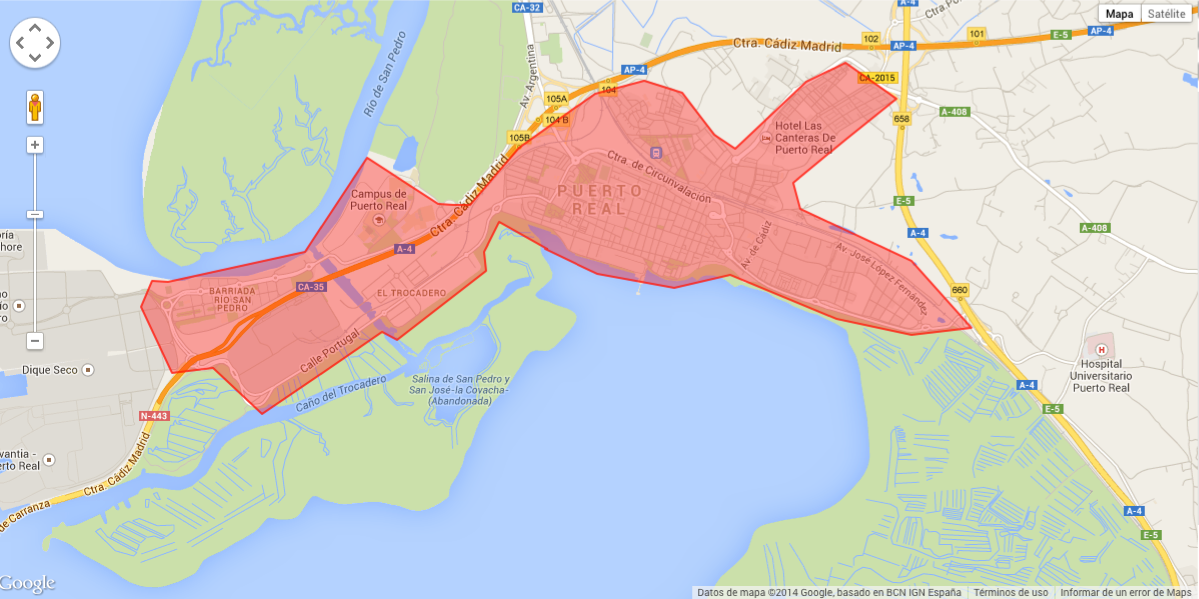
\includegraphics[scale=0.3]{zona-urbana.png} 
\caption{Acotamiento de mapa para la zona urbana del municipio.}
\end{figure}	

\begin{figure}[H]
\centering
	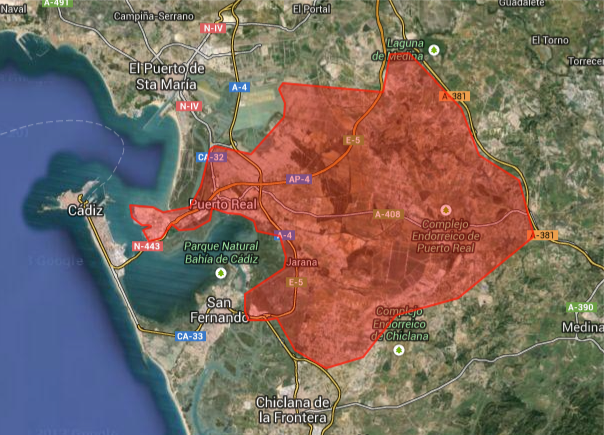
\includegraphics[scale=0.5]{termino-municipal.png} 
\caption{Acotamiento de mapa para la totalidad del municipio.}
\end{figure}

De este polígono se obtiene una serie de vértices con el formato ( \textbf{latitud} , \textbf{longitud} ) que serán cargados cuando el usuario desee establecer el puto de su domicilio al solicitar la recogida de muebles y enseres. De esta forma se puede averiguar cuando se obtenga una coordenada si se encuentra dentro de la zona de servicio y si corresponde a una zona urbana o no. El formato de los ficheros xml incluidos en la app móvil es el siguiente:

% Código en que se explica como se ha ellaborado el fichero xml con las ubicaciones
\begin{lstlisting}[style=XML]
<?xml version="1.0" encoding="UTF-8" ?>
<zone>
  <item>
    <latitude>36.48038014291644</latitude>
    <longitude> -6.178951263427734</longitude>
  </item>
  <item>
    <latitude>36.47085575451313</latitude>
    <longitude> -6.179466247558594</longitude>
  </item>
  ...
</zone>
\end{lstlisting}
